\documentclass[a4paper,12pt]{article}
\usepackage[utf8]{inputenc}
\usepackage{graphicx}
\usepackage{geometry}
\usepackage{hyperref}
\usepackage{listings}
\usepackage{xcolor}
\geometry{margin=1in}

\title{\textbf{Dokumentacja Techniczna Projektu Helpdesk}}
\author{Autor: Tomasz Myszak}
\date{\today}

\begin{document}

\maketitle

\tableofcontents
\newpage

% Sekcja: Opis projektu
\section{Opis projektu}
Projekt \textbf{Helpdesk} jest aplikacją wspierającą organizację w obsłudze zgłoszeń serwisowych (tzw. ticketów) oraz zarządzaniu bazą wiedzy. Głównym celem systemu jest usprawnienie komunikacji między pracownikami a działem wsparcia IT oraz dostarczanie szybkich rozwiązań problemów.

\subsection{Cel projektu}
\begin{itemize}
    \item Ułatwienie rejestrowania i śledzenia zgłoszeń przez pracowników.
    \item Szybsze rozwiązywanie problemów dzięki systematyzacji wiedzy.
    \item Efektywne zarządzanie zgłoszeniami przez administratorów IT.
\end{itemize}

\subsection{Zakres projektu}
System składa się z dwóch głównych modułów:
\begin{enumerate}
    \item \textbf{System zgłoszeń (Ticketing System)} -- rejestrowanie, przypisywanie i zarządzanie zgłoszeniami.
    \item \textbf{Baza wiedzy} -- gromadzenie i wyszukiwanie artykułów z rozwiązaniami problemów.
\end{enumerate}

\newpage

% Sekcja: Wymagania funkcjonalne
\section{Wymagania funkcjonalne}
\begin{enumerate}
    \item \textbf{Zarządzanie zgłoszeniami (Ticketing System)}
    \begin{itemize}
        \item Tworzenie zgłoszeń z tytułem, opisem, priorytetem i załącznikami.
        \item Przeglądanie i filtrowanie zgłoszeń przez administratorów.
        \item Zmiana statusu zgłoszeń: otwarte, w trakcie realizacji, zamknięte.
    \end{itemize}

    \item \textbf{Obsługa załączników}
    \begin{itemize}
        \item Możliwość dodawania plików do zgłoszeń.
        \item Przechowywanie plików na serwerze.
    \end{itemize}

    \item \textbf{Zarządzanie bazą wiedzy}
    \begin{itemize}
        \item Tworzenie, edytowanie i usuwanie artykułów z instrukcjami.
        \item Wyszukiwanie artykułów po tagach lub pełnym tekście.
    \end{itemize}

    \item \textbf{Autoryzacja i role użytkowników}
    \begin{itemize}
        \item Role: pracownik, administrator.
        \item Logowanie i autoryzacja użytkowników.
    \end{itemize}

    \item \textbf{Statystyki i raportowanie}
    \begin{itemize}
        \item Wyświetlanie statystyk zgłoszeń: liczba zgłoszeń, średni czas odpowiedzi.
    \end{itemize}
\end{enumerate}

\newpage

% Sekcja: Wymagania niefunkcjonalne
\section{Wymagania niefunkcjonalne}
\begin{itemize}
    \item \textbf{Wydajność:} System powinien obsługiwać do 500 użytkowników jednocześnie.
    \item \textbf{Bezpieczeństwo:} Dane użytkowników i zgłoszeń muszą być zabezpieczone (SSL/TLS, autoryzacja JWT).
    \item \textbf{Skalowalność:} Możliwość rozszerzenia systemu o nowe funkcjonalności.
    \item \textbf{Dostępność:} System dostępny 24/7.
    \item \textbf{Przenaszalność:} Wsparcie dla kontenerów Docker oraz hostingu w chmurze Azure.
\end{itemize}

\newpage

% Sekcja: Diagramy UML
\section{Diagramy UML}

\subsection{Diagram przypadków użycia}
\begin{center}
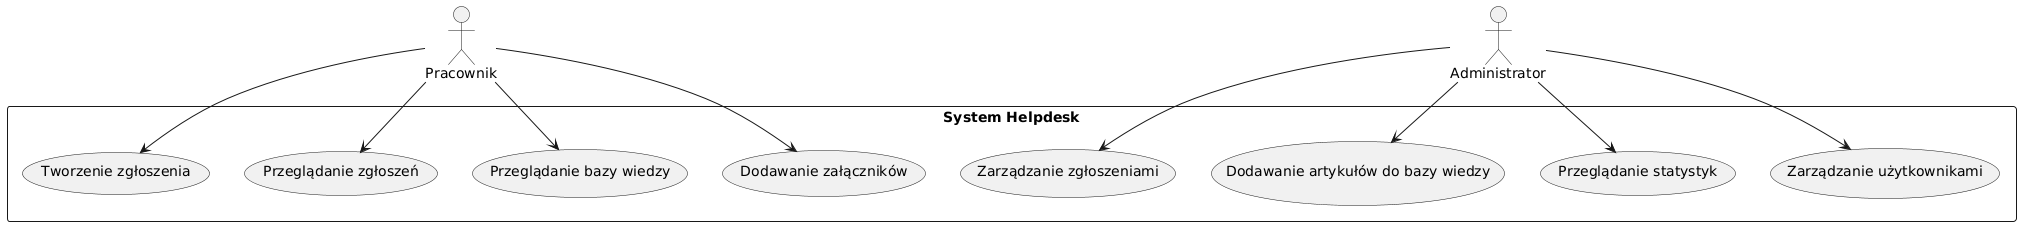
\includegraphics[width=0.8\textwidth]{draw/diagramPU.png}
\end{center}

\subsection{Diagram Klass}
\begin{center}
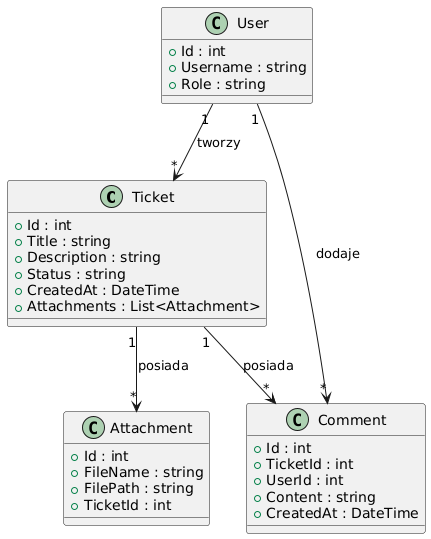
\includegraphics[width=0.8\textwidth]{draw/diagramClass.png}
\end{center}


\subsection{Diagram Aktywnosci}
\begin{center}
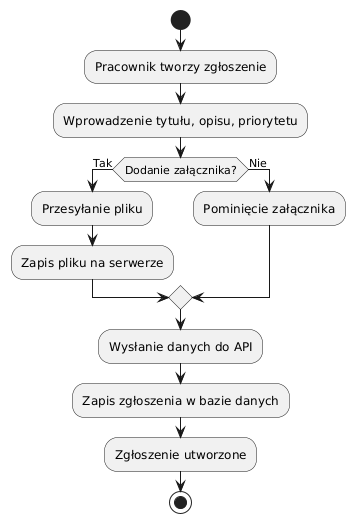
\includegraphics[width=0.8\textwidth]{draw/diagramAktywnosci.png}
\end{center}

\subsection{Diagram komponetnów}
\begin{center}
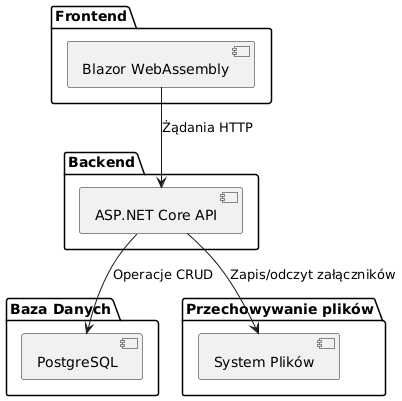
\includegraphics[width=0.8\textwidth]{draw/diagramKomponentow.png}
\end{center}

\subsection{Diagram sekwencji}
\begin{center}
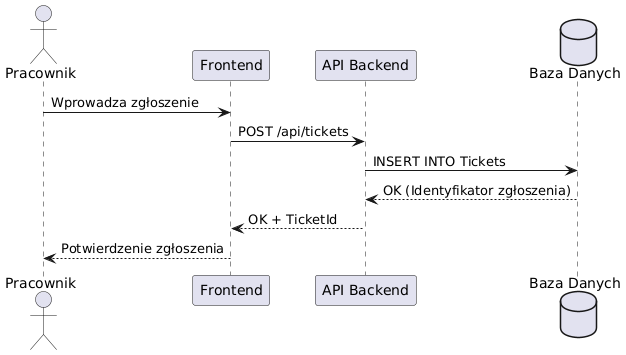
\includegraphics[width=0.8\textwidth]{draw/diagramSekwencji.png}
\end{center}

\newpage

\subsection{Diagram sekwencji (przykład dodawania zgłoszenia)}
\begin{lstlisting}[language=PlantUML, caption=Kod PlantUML dla diagramu sekwencji]
@startuml
actor User
participant "Frontend" as FE
participant "API" as BE
database "Database" as DB

User -> FE: Dodaj zgłoszenie
FE -> BE: POST /api/tickets
BE -> DB: Insert zgłoszenie
DB --> BE: OK
BE --> FE: OK + TicketId
FE --> User: Potwierdzenie
@enduml
\end{lstlisting}

\newpage

% Sekcja: Architektura systemu
\section{Architektura systemu}
System oparty jest na architekturze **klient-serwer**:
\begin{itemize}
    \item \textbf{Frontend:} Blazor WebAssembly.
    \item \textbf{Backend:} ASP.NET Core Web API.
    \item \textbf{Baza danych:} PostgreSQL.
    \item \textbf{Przechowywanie plików:} System plików na serwerze.
    \item \textbf{Hosting:} Azure App Service lub Docker.
\end{itemize}

\begin{center}
\includegraphics[width=0.8\textwidth]{system_architecture.png}
\end{center}

\newpage

% Sekcja: Podsumowanie
\section{Podsumowanie}
Aplikacja Helpdesk zapewnia kompleksowe wsparcie dla organizacji w zakresie zarządzania zgłoszeniami oraz budowania bazy wiedzy. Dzięki nowoczesnym technologiom, takim jak ASP.NET Core i Blazor, system jest wydajny, skalowalny i bezpieczny.

\end{document}
